%\section*{Why we tried this}
The first model we considered was a seq2seq (sequence-to-sequence) model.
It resembles the one mention in \cite{denkowski:lavie:meteor-wmt:2014}. 
While this architecture is usually used for language translation, it happens to also be widely used for chatbot creation. 
The success the seq2seq model has had in other chatbot implementations we researched, along with it's easy implementation in Keras is why this architecture was chosen.
In this section we discuss how we developed, trained and analyzed this model.

\subsection{Data Preparation}
%\begin{figure}
%\begin{python}
%	keepPunct = '[.,!?;]'
%	re.findall(r"[\w]+|"+keepPunct, 
%	'This is a test. Is this test 2?')
%	>>['This','is','a','test','.','Is','this','test','?']
%\end{python}
%\caption{Example of preprocessing statement for seq2seq model.}
%\label{fig:preprocess_s2s}
%\end{figure}
%\begin{python}
%	>>['<START> This is a test . Is this test ? <END>']
%\end{python}
Our first step was further reprocessing our datasets so that we could train on it.
We decided to do the following preprocessing steps:
%We break this process into the following steps:
We broke the dialogue into words  and punctuation mark. 
A word here does not have to reference and actual English word but a maximal sequence of characters excluding punctuation marks and white space. 
We decided that treating the punctuation marks as individual tokens would hopefully allow our model to better understand questions, statements and commands.
We also removed numerical data since smaller numbers were consistently represented by their word form and larger numbers seemed too rarely appear in the raw data.
This seemed like a easy way to reduce our vocabulary.
Finally we add a start and end tags to each statement.

To make the above data ingestible for the embedding layer of our model and easier to work with in general, every word, punctuation mark and tag was mapped to a numeric token. 
The \emph{tokenizer} consumes the entire corpus to create this mapping which is then applied to every statement and response in our dataset to create a collection of input and output sequence pairs.
The next was \emph{padding} the tokenized sequences with zeroes so they all have the same size.
%This was done by finding the longest sequence and padding all other sequences with zeros to have the same length as the longest sequence.
The input sequences were pre padded while the output was post padded.
%\begin{itemize}
%    \item When the sentence being processed is an output sentence a start and end token are added to the sentence.
%
%
%
%
%    
%\begin{python}
%    tokenizer = keras.preprocessing.text.Tokenizer(filters='\t\n',
%                                                   oov_token='<UNK>', 
%                                                   lower=False)
%    tokenizer.fit_on_texts(inputs + outputs)
%    tokenizer.texts_to_sequences(['This is a test input .',
%                        '<START> This is another test output . <END>'])
%    >>[[1,2,3,4,5,8],[10, 1, 2, 6, 4, 7, 8, 11]]
%\end{python}
%
%    \item 
%\end{itemize}
%\begin{python}
%    inputSequences = [[1,2,4,8],[2,4,3]]
%    ouputSequences = [[10, 1, 2, 6, 11], [10, 1, 2, 11]]
%    paddedInputs = preprocessing.sequence.pad_sequences(inputSequences,
%                                                     maxlen=maxInputLen,
%                                                     padding='pre' )
%    paddedOutputs = preprocessing.sequence.pad_sequences(ouputSequences,
%                                                     maxlen=maxOutputLen,
%                                                     padding='post' )
%    paddedInputs
%    >>[[1,2,4,8],[0,2,4,3]]
%    paddedOutputs
%    >>[[10, 1, 2, 6, 11], [10, 1, 2, 11,0]]
%\end{python}

Next, every token in the sequence had to be given a unique vector representation \cite{DBLP:journals/corr/MikolovSCCD13}. 
This was handle by a \textbf{keras.layers.Embedding} layer. 
To provide contextual representations of tokens (words, punctuation marks and tags), \textbf{GloVe 300-dimensional word embeddings} were used to initialized the embedding layer weights. 
Since the model outputs a \emph{softmaxed} prediction on each token, the next step involved converting output tokens to \emph{one-hot vectors}. 
Since the goal of the decoder was to predict the next token given the current token, the tokenized output sequence was shifted to the left by one step before being converted to one-hot vectors.  
%
%\begin{python}
%    #If the vocabulary was of size 3
%    paddedOutputs = [1,2,3,0]
%    paddedOutputs = paddedOutputs[1:] #left shift step
%    onehotOutput = keras.utils.to_categorical( paddedOutputs , 3+1)
%    onehotOutput
%    >>[[0,1,0,0],[0,0,1,0],[0,0,0,1],[1,0,0,0]]
%\end{python}

\subsection{The Model}
\begin{figure}
	\begin{center}
		\fbox{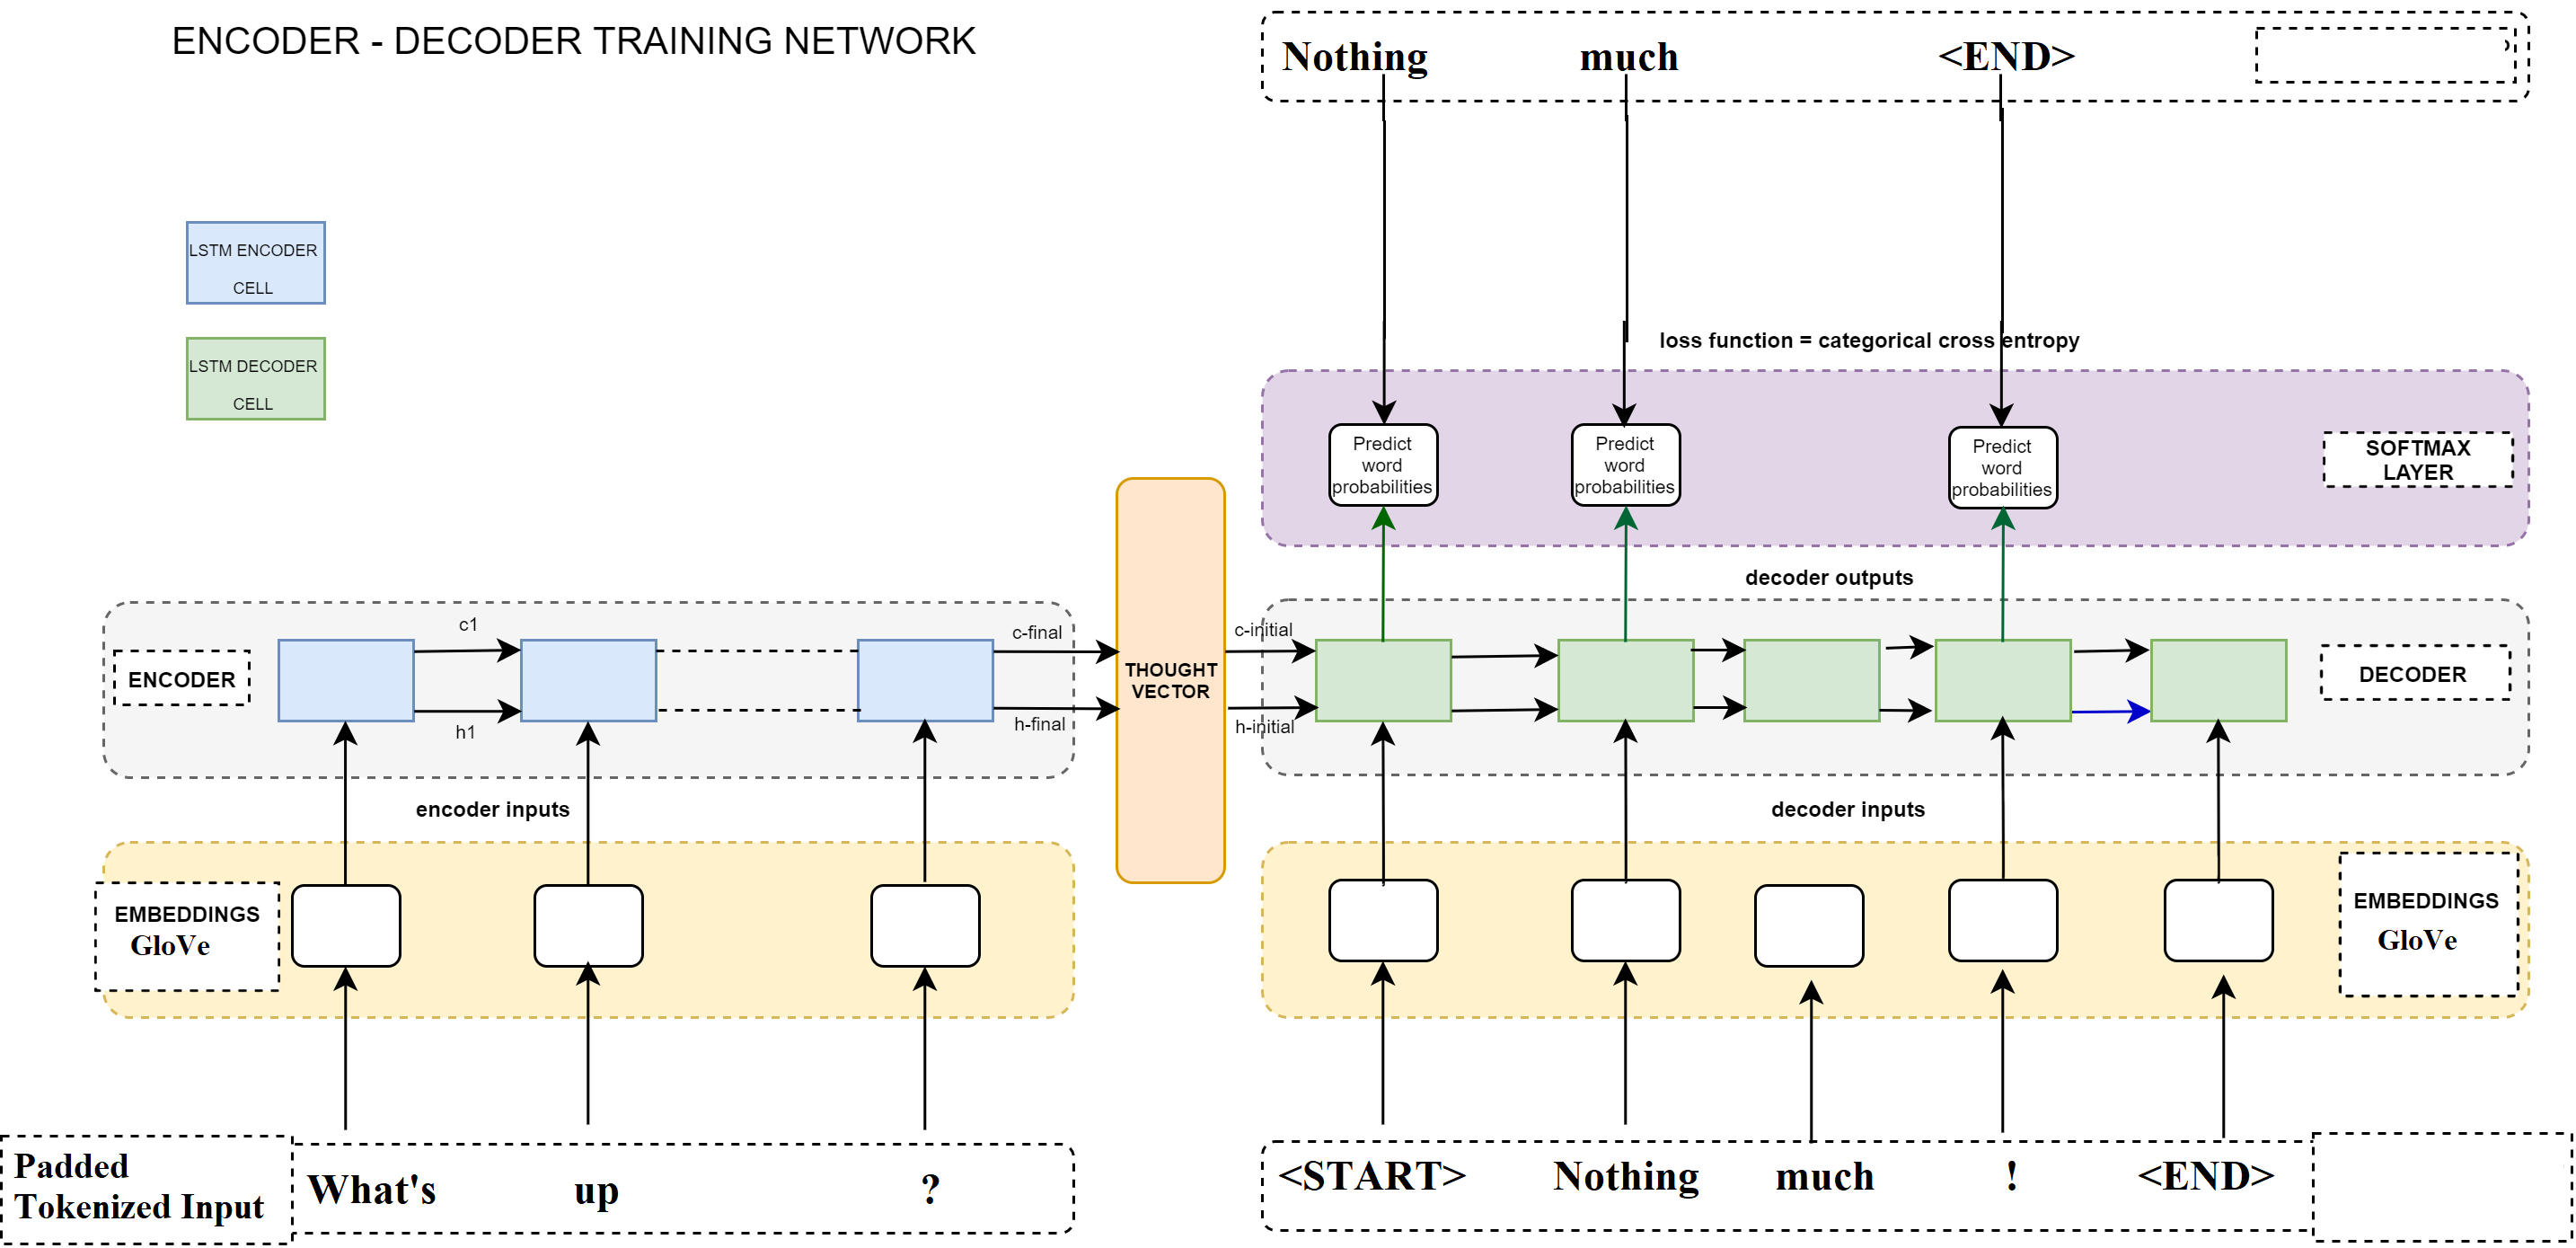
\includegraphics[width=\textwidth]{seq2seqModel.png}}
	\end{center}
	\caption{A diagram of our seq2seq model. Image edit from original image found \url{https://github.com/samurainote/Automatic-Encoder-Decoder_Seq2Seq_Chatbot.}}
	\label{fig:s2s_model}
\end{figure}
The model consists of an Encoder and a Decoder.
Padded input token sequences are converted to a sequence of word embeddings using a \textbf{Keras.embedding.layer} as described above.
Each of these word vectors are fed to the \textbf{keras.layers.LSTM} \emph{encoder long short-term memory} (LSTM) one at a time. 
The encoder LSTM tries to capture the essence of the encoded input sequence in two \emph{thought vectors}, the \emph{output context vector} and the \emph{hidden state vector}.
Both thought vectors are then passed to the decoder (See Figure \ref{fig:s2s_model}).

The \emph{decoder LSTM} is fed a padded sequence of output word embeddings along with the two thought vectors.
The decoder model is trained to use a \emph{dense SoftMax} output layer \textbf{keras.layers.Dense} with activation \textbf{keras.activations.softmax} to predict the most likely output word among all words in the vocabulary.
Once the model is trained, an \emph{inference encoder and decoder model} is created using the trained model weights. 
The inference encoder model takes in statement and two generated state vectors. 
The input state vectors are fed into the inference decoder model along with a sentence start tag. 
All words predicted by the SoftMax layer are captured until an end tag is generated (See Figure \ref{fig:s2s_model_decoder}).

\begin{figure}
	\begin{center}
		\fbox{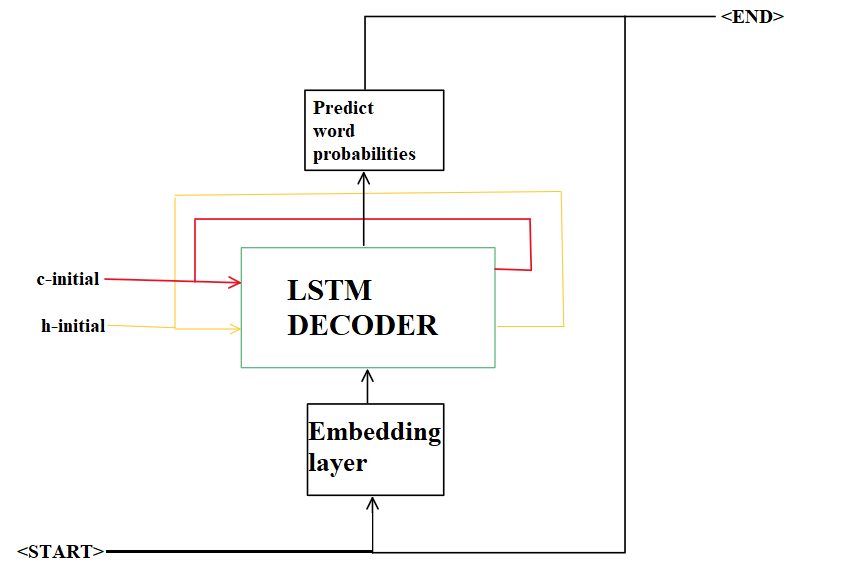
\includegraphics[width=.9\textwidth]{inference.png}}
	\end{center}
	\caption{A diagram of our seq2seq model's decoder.}
	\label{fig:s2s_model_decoder}
\end{figure} 

\subsection{Performance and Error Analysis}

\begin{figure}
\begin{center}
	\scalebox{.8}
	{
	\begin{tabular}{ |l|c|c|c|c|c|c|c| } 
		\hline
		\textbf{Dataset} & \textbf{BLEU Avg. Score} & \textbf{ROUGE-1 Score} & \textbf{ROUGE-$\ell$} & \textbf{METEOR Score} & \textbf{WER Avg.} & \textbf{Human Eval.}\\
		\hline
		Q\&A & $0.0530$ & $0.213$ & $0.204$ & $0.092$ & $1.554$ & $0.413$\\
		\hline
		Joey & $0.015$ & $0.141$ & $0.131$ & $0.064$ & $1.922$ & $0.350$\\ 
		\hline
	\end{tabular}
	}
\end{center}
\label{fig:s2s_data}
\caption{Table showing various scores for this sequence-to-sequence model on the Joey and generic questions and answers dataset (Q\&A).}
\end{figure}

As seen in Figure \ref{fig:s2s_data} this model did not perform well with respect to most of the automatic metrics.
This is somewhat to be expected though given that these types of metrics are known to be flawed when evaluating our kind of task.
We will discuss this in greater detail in Section \ref{sec:conclusion}.
We also note some success in this model for the human evaluation.
Again, these numbers may be slightly higher than expected due to the lack of preprocessing of our original dataset.
That is, some of it may be based on the human tester randomly picking between two poor responses to a statement and not necessary two equally good responses. 
We will also review this in greater detail in Section \ref{sec:conclusion}.

Here will review a few particular cases where this model consistently failed to perform well on human metrics and follow with some ideas for future improvement.

\subsection{Pitfalls and Improvements}
One major pitfall faced while developing the seq2seq model was during training of our model. 
Specifically we initially had trouble providing the model with one-hot output vectors. 
As discussed above, the model uses a output softmax layer to predict the best possible word output. 
This means the length of each training output vector equals the length of the vocabulary of the entire corpus. 
This is multiplies by the number of tokens (words, punctuation marks and tags) in the sequence and this is then further multiplied by the number of training data points. 
With a vocabulary size of $3000$, a sequence length of $100$ and training data size of $7000$, the size of the entire output training data become $3000*100*7000$. 
This is too large of a matrix to store in memory. 
This problem was fixed by training in batches.
This was implemented using the Keras $fit\_generator$ function along with our own custom data generation function. 

One way we were able to imporove our model's performance was to change how we do our token embedding.
The initial model randomly generated embedding vectors of tokens. 
This did give good results as the word embedding held no information regarding the tokens they represented. 
This problem was fixed using GloVe word embedding that contextually represented the words they were associated to.
 
% During development, while training on a large number of epochs, a single failure in training lead to the loss of all training progress as the model was saved only in the end of training. 
% This was fixed by creating a custom Keras callback to save the model every specified number of epochs.
%\end{itemize}
%\section*{Future improvements}
While the current model seems to learn Joey like responses to some extent, it fails to understand how English sentences are structured. 
This leads to a lot of generated responses failing tests as they are eliminated for not looking like English sentences. 
We believe this can be fixed by adding a \emph{conditional random field (CRF)} layer using the Viterbi algorithm.
Hopefully this would give the model a better sense of English sentence structure. 
%This way a model know that an adverb comes after a verb etc. thereby facilitating the generation of English like sentences.
   
Another issue we noticed was that this model currently takes an argmax of the output predictions to choose the most probable word. 
Using a \emph{beam search} across predictions instead of just an argmax could improve prediction results.
    
The current model used just two fixed length vectors to represent the entire input sequence. 
When input sequence are really long, two fixed length vectors may not be enough to capture its entire essence. 
Attention could help solve this issue. 
The technique was tried but could not be successfully implemented due to the time constraint. 
Adding attention to models like this one has been show to drastically improve performance of the model when the input sentences are long.